%==============================================================================
%  MATH 231 -- Linear Algebra I (Queens College, Fall 2026)
%  VECTOR CALCULUS UNIT, PART 2 -- n Dimensions, the Jacobian, and the Hessian
%
%  SECTION NUMBERING CONTINUES from Part 1.  The unit runs:
%      Part 1  MATH231_veccalc_1_derivatives_and_the_gradient   Sections 1-9
%      Part 2  MATH231_veccalc_2_n_dimensions_and_the_hessian   Sections 10-15
%  Hence the \setcounter{section}{9} below: this part opens at Section 10.
%  Definitions and examples are numbered BY SECTION so they are unique across
%  the whole unit.  References to Sections 1-9 point into Part 1.
%
%  The unit numbering still does NOT continue from the vector unit (Sec. 1-24),
%  the computational unit, or the matrix unit.
%
%  WHAT THIS PART IS FOR.  Part 1 did the whole subject for f : R^2 -> R, and
%  did it with pictures.  This part does two things and only two:
%
%    (1) Sec. 10-13 LIFT Part 1 from the plane to R^n.  These are deliberately
%        brisk.  Every definition here is a Part 1 definition with n in place of
%        2, every proof is the Part 1 proof unchanged, and the text says so
%        rather than re-deriving.  The ONE genuinely new ingredient is e_j,
%        which lets the n coordinate-wise limits of Part 1's Sec. 6.1 be
%        written as a single formula.  Do not pad these sections out; their
%        pedagogical point IS that nothing changes.
%    (2) Sec. 14-15 are new material with no Part 1 counterpart: vector-valued
%        functions, the Jacobian, and the Hessian.
%
%  SEC. 15 CLOSES A LOOP OPENED IN SEC. 12.1.  That section records the
%  signature grad f : R^n -> R^n and leaves it.  Sec. 14.3 collects it: the
%  gradient is itself a vector-valued function, so it has a Jacobian, and that
%  Jacobian IS the second derivative.  The Hessian therefore arrives as a
%  consequence of a signature already on the page rather than as a new
%  definition.
%
%  INDEX CONVENTION for the Hessian, stated once in Sec. 15.1 and used
%  throughout: (H_f)_ij = d/dx_i ( df/dx_j ).  Under Clairaut the two orders
%  agree, so the choice is immaterial to the answer -- but it must be FIXED
%  before Clairaut is stated, or the symmetry claim in Sec. 15.3 has no content.
%
%  THE JACOBIAN EXAMPLE in Sec. 14.2 is deliberately non-symmetric (2x, -2y over
%  2y, 2x) so that Sec. 15.3's symmetry claim reads as a real restriction rather
%  than a property of matrices of partial derivatives in general.
%
%  PREREQUISITES BEYOND PART 1.  This part uses material Part 1 deliberately
%  avoided: R^n and the standard basis e_1,...,e_n (vector unit Sec. 16 and
%  Sec. 24.1, i.e. vectors Parts 4 and 5), and matrices, transpose and symmetry
%  (matrix unit Sec. 6.5).  Do not move any of that back into Part 1.
%
%  LANGUAGE DELIBERATELY AVOIDED, as in Part 1: "continuously differentiable",
%  "smooth", "class C^1".  The one place continuity is genuinely load-bearing
%  is Clairaut's hypothesis in Sec. 15.2, where it is stated in words.
%
%  AUDIENCE: distributed to students.  No instructor-facing apparatus.
%
%  Compile with pdflatex (standard TeX Live packages only; uses tikz).
%==============================================================================
\documentclass[11pt]{article}

\usepackage[margin=1in]{geometry}
\usepackage{amsmath,amssymb,amsthm}
\usepackage[dvipsnames]{xcolor}
\usepackage{enumitem}
\usepackage{booktabs}
\usepackage{array}
\usepackage[hidelinks]{hyperref}
\usepackage{titlesec}
\usepackage{needspace}
\usepackage{tikz}
\usetikzlibrary{arrows.meta,calc}

%------------------------------------------------------------------ style ----
\titleformat{\section}{\large\bfseries\sffamily}{\thesection.}{0.6em}{}
\titleformat{\subsection}{\normalsize\bfseries\sffamily}{\thesubsection.}{0.5em}{}
\titlespacing*{\section}{0pt}{14pt}{6pt}

\theoremstyle{plain}
\newtheorem{thm}{Theorem}[section]

\theoremstyle{definition}
\newtheorem{defn}{Definition}[section]
\newtheorem{ex}{Example}[section]
\theoremstyle{remark}
\newtheorem*{rmk}{Remark}
\newtheorem*{warn}{A common confusion}

\newcommand{\lookahead}{\par\smallskip\noindent
  \textbf{\sffamily\textcolor{RoyalBlue}{Looking ahead.}}\ \ignorespaces}
\newcommand{\lookback}{\par\smallskip\noindent
  \textbf{\sffamily\textcolor{ForestGreen}{From the vector unit.}}\ \ignorespaces}

%--------------------------------------------------------------- notation ----
\newcommand{\R}{\mathbb{R}}
\newcommand{\vc}[1]{\mathbf{#1}}
\newcommand{\norm}[1]{\lVert #1\rVert}
\newcommand{\ip}[2]{\langle #1,\, #2\rangle}
\newcommand{\grad}{\nabla}
\newcommand{\pd}[2]{\frac{\partial #1}{\partial #2}}
\newcommand{\dd}[2]{\frac{d #1}{d #2}}
\newcommand{\mt}[1]{\mathbf{#1}}          % matrices: bold upper case
\newcommand{\T}{^{\mathsf{T}}}            % transpose
\newcommand{\pdd}[3]{\frac{\partial^{2} #1}{\partial #2\,\partial #3}}

%------------------------------------------------------------- tikz helpers --
\tikzset{
  axisline/.style = {->, gray!75, thin},
  curveln/.style  = {RoyalBlue, very thick},
  vecarr/.style   = {-{Stealth[length=2.6mm,width=2.0mm]}, very thick}
}

\setcounter{section}{9}   % this part opens at Section 10; see the header note

\title{\vspace{-1.2cm}\textbf{\sffamily MATH 231 -- Linear Algebra I}\\[4pt]
       {\large\sffamily The Vector Calculus Unit, Part 2 \textbullet\
        $n$ Dimensions, the Jacobian, and the Hessian}\\[2pt]
       {\normalsize\sffamily Kiely Hall 326 \textbullet\
        Instructor: Kevin Bedoya}}
\author{}
\date{}

\begin{document}
\maketitle
\vspace{-1.6cm}

\noindent\textbf{About this document.} Part 1 of this unit developed the whole
of differential calculus for functions $f:\R^{2}\to\R$: the two partial
derivatives, the gradient, the directional derivative, steepest ascent, and the
linear approximation. It stayed in the plane so that every statement could be
drawn.

This part does two things. Sections \S10--\S13 lift all of that to $\R^{n}$, and
they are short on purpose --- the point is that almost nothing changes. Every
definition is a Part 1 definition with $n$ in place of $2$; every argument is a
Part 1 argument copied out. The single new ingredient is a piece of notation
that lets $n$ separate limits be written as one.

Sections \S14--\S15 are new. Differentiating $f:\R^{n}\to\R$ produced the
gradient, which is \emph{not} a function of the same type as $f$ --- so
differentiating a second time needs a derivative for functions with vector
output. That is the Jacobian, and applying it to the gradient produces the
Hessian: the second derivative of a scalar function of $n$ variables, which
turns out to be a matrix.

\begin{warn}[Section numbers]
This part continues the numbering of Part 1, so it opens at \S10. A bare
``\S12'' below means \S12 \emph{of this unit}, not of the vector unit, which
also has a \S12. Whenever another unit is meant, it is named.
\end{warn}

\medskip
\noindent\textbf{Assumed.} All of Part 1. From the vector unit: $\R^{n}$ and its
vectors (\S24.1); the standard basis vectors $\vc{e}_1,\dots,\vc{e}_n$ (\S16,
\S24.1); the dot product and the identity
$\ip{\vc{u}}{\vc{v}}=\norm{\vc{u}}\norm{\vc{v}}\cos\theta$ (\S11.3); and the
Euclidean norm (\S2). From the matrix unit: matrices, the transpose, and what it
means for a matrix to be symmetric (\S6.5).

\medskip
\noindent\textbf{What you should be able to do afterwards.} Read the signature
$f:\R^{n}\to\R$; write the partial derivative as a single limit using
$\vc{e}_j$; assemble the $n$ partials into a gradient and compute one; state the
directional derivative and the steepest-ascent property in $\R^{n}$ and say why
the Part 1 argument needed no change; write the linear approximation in $n$
variables; say what a function $\R^{n}\to\R^{m}$ is; build its Jacobian and read
its shape; explain why the gradient has a Jacobian of its own; build the Hessian
of a scalar function; state Clairaut's theorem and the role of its hypothesis;
and say why the Hessian is symmetric when a general Jacobian is not.
%==============================================================================
\section{From the plane to \texorpdfstring{$\R^{n}$}{Rn}}
%==============================================================================

%------------------------------------------------------------------------------
\subsection{The signature}
%------------------------------------------------------------------------------
\begin{defn}[Scalar function of $n$ variables]
A \textbf{scalar function of $n$ variables} is a function
\[
  f:\R^{n}\longrightarrow\R ,
\]
taking a vector $\vc{x}=[\,x_1,x_2,\dots,x_n\,]\in\R^{n}$ and returning a single
real number $f(\vc{x})$.
\end{defn}

\noindent This is \S5.1 with $n$ in place of $2$, and nothing else is different:
the input is a vector, the output is a scalar, and such functions are still
called \textbf{scalar fields}. What is lost is the picture. A function
$\R^{2}\to\R$ has a graph in three dimensions --- a surface --- and every
statement of Part 1 could be checked against it. For $n=3$ the graph would need
four dimensions, and there is no drawing it.

That loss is worth naming, because it is the reason this part is organised the
way it is. The formulas survive; the pictures do not. When you want to know what
a statement about $\R^{n}$ \emph{means}, set $n=2$, draw it, and trust that the
algebra says the same thing with more coordinates.

%------------------------------------------------------------------------------
\subsection{Examples}
%------------------------------------------------------------------------------
\begin{ex}
Each of the following is a function $\R^{n}\to\R$.

\smallskip
\noindent\textbf{(a)} $f(x,y,z)=x^{2}+y^{2}+z^{2}$, with $n=3$. Three inputs,
still one output.

\smallskip
\noindent\textbf{(b)} $f(\vc{x})=\norm{\vc{x}}=\sqrt{x_1^{2}+\cdots+x_n^{2}}$,
for any $n$. The Euclidean norm eats a vector and returns its length, a single
number (vector unit \S2, \S24.1).

\smallskip
\noindent\textbf{(c)} $f(\vc{x})=\ip{\vc{a}}{\vc{x}}=a_1x_1+\cdots+a_nx_n$ for a
fixed vector $\vc{a}\in\R^{n}$. The dot product against a fixed vector is
likewise $\R^{n}\to\R$ (vector unit \S11.3).

\smallskip
\noindent\textbf{(d)} The temperature at each point of a room: $n=3$. The
closing price of each of $500$ stocks fed into a single portfolio value:
$n=500$, and no picture at all.
\end{ex}

\begin{rmk}
Examples (b) and (c) were already on the list in \S5.2 for $n=2$. They are
listed again because they are the two functions $\R^{n}\to\R$ you will meet most
often, and because their gradients, computed in \S12.2, are worth knowing by
heart.
\end{rmk}

%------------------------------------------------------------------------------
\subsection{Stepping in one coordinate direction}
%------------------------------------------------------------------------------
Part 1 defined the two partial derivatives with two separate limits, one
displacing $x$ and one displacing $y$:
\[
  \lim_{h\to0}\frac{f(x+h,\;y)-f(x,y)}{h},
  \qquad
  \lim_{h\to0}\frac{f(x,\;y+h)-f(x,y)}{h} .
\]
Writing $n$ of those out, one per coordinate, is unworkable past about three. The
vector unit supplies exactly the notation needed to collapse them into one.

\lookback $\vc{e}_j$ is the $j$-th standard basis vector of $\R^{n}$: a $1$ in
slot $j$ and $0$ everywhere else (vector unit \S16, \S24.1). So
\[
  \vc{x}+h\,\vc{e}_j
  = [\,x_1,\;\dots,\;x_{j-1},\;x_j+h,\;x_{j+1},\;\dots,\;x_n\,] :
\]
adding $h\vc{e}_j$ changes the $j$-th coordinate by $h$ and leaves every other
coordinate exactly where it was.

That is the whole of the new notation. In $\R^{2}$, $\vc{e}_1=[\,1,\,0\,]$ and
$\vc{e}_2=[\,0,\,1\,]$, so $\vc{x}+h\vc{e}_1=(x+h,\,y)$ and
$\vc{x}+h\vc{e}_2=(x,\,y+h)$ --- the two displacements Part 1 wrote out by hand.

%==============================================================================
\section{Partial derivatives in \texorpdfstring{$n$}{n} variables}
%==============================================================================

%------------------------------------------------------------------------------
\subsection{The definition}
%------------------------------------------------------------------------------
\begin{defn}[Partial derivative]
Let $f:\R^{n}\to\R$. The \textbf{partial derivative of $f$ with respect to
$x_j$} at the point $\vc{x}$ is
\begin{equation}\label{eq:partialn}
  \pd{f}{x_j}(\vc{x})
  \;=\;\lim_{h\to0}\frac{f(\vc{x}+h\,\vc{e}_j)-f(\vc{x})}{h},
\end{equation}
provided the limit exists.
\end{defn}

\noindent One formula now covers all $n$ of them. Setting $n=2$ and $j=1$
recovers the first of the two limits displayed in \S10.3, and $j=2$ recovers the
second; no content was added in passing from two variables to $n$, only
notation.

\begin{center}
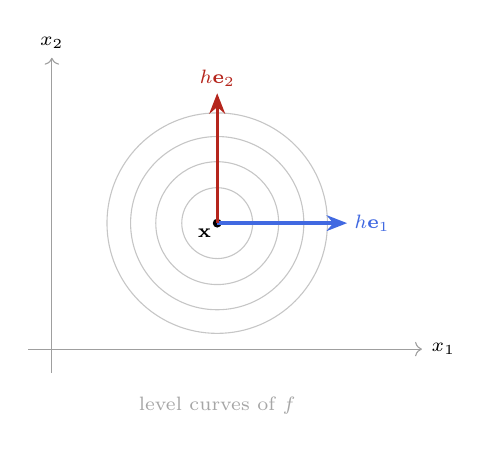
\begin{tikzpicture}[scale=1.0]
  \draw[axisline] (-0.3,0) -- (4.7,0) node[right,font=\scriptsize,black]{$x_1$};
  \draw[axisline] (0,-0.3) -- (0,3.7) node[above,font=\scriptsize,black]{$x_2$};
  \foreach \r in {0.45,0.78,1.10,1.40}
    { \draw[gray!45] (2.1,1.6) circle (\r); }
  \fill[black] (2.1,1.6) circle (1.6pt);
  \node[below left,font=\scriptsize,inner sep=2pt] at (2.1,1.6) {$\vc{x}$};
  \draw[vecarr,RoyalBlue] (2.1,1.6) -- (3.75,1.6)
        node[right,font=\scriptsize,inner sep=2pt]{$h\vc{e}_1$};
  \draw[vecarr,BrickRed]  (2.1,1.6) -- (2.1,3.25)
        node[above,font=\scriptsize,inner sep=2pt]{$h\vc{e}_2$};
  \node[font=\scriptsize,gray!70] at (2.1,-0.72) {level curves of $f$};
\end{tikzpicture}
\end{center}

\noindent The figure can only be drawn for $n=2$, where there are two arrows. For
general $n$ there are $n$ of them, mutually orthogonal, and the picture is gone
--- but \eqref{eq:partialn} is unchanged.

\begin{rmk}[What the geometric reading becomes]
Part 1's \S6.2 read $\partial f/\partial x$ as the slope of a slice: hold $y=b$,
cut the surface with that vertical plane, and take the ordinary tangent slope of
the resulting curve. The same reading survives verbatim. Fixing every coordinate
but $x_j$ turns $f$ into a one-variable function
\[
  g(t) \;=\; f(x_1,\dots,x_{j-1},\,t,\,x_{j+1},\dots,x_n),
\]
and $\partial f/\partial x_j(\vc{x})$ is $g'(x_j)$. What is lost is only the
ability to draw the slice, not the fact that it is one.
\end{rmk}

%------------------------------------------------------------------------------
\subsection{Computing them}
%------------------------------------------------------------------------------
The rule of \S6.3 is unchanged, and for the same reason: every variable except
$x_j$ is held fixed, so they behave as constants and the expression becomes a
function of the one live variable.

\begin{center}
\fcolorbox{RoyalBlue!45}{RoyalBlue!7}{%
\begin{minipage}{0.9\textwidth}
\centering
To compute $\partial f/\partial x_j$: treat every variable other than $x_j$ as a
constant, and differentiate as in one-variable calculus.
\end{minipage}}
\end{center}

\begin{ex}
Let $f(x,y,z)=x^{2}y+y^{2}z+z^{2}x$. Three variables, so three partials. For
each, two of the three are constants:
\[
  \pd{f}{x}=2xy+z^{2},
  \qquad
  \pd{f}{y}=x^{2}+2yz,
  \qquad
  \pd{f}{z}=y^{2}+2zx .
\]
\end{ex}

\begin{ex}
Let $f(\vc{x})=\ip{\vc{a}}{\vc{x}}=a_1x_1+\cdots+a_nx_n$, example (c) of \S10.2.
Only the $j$-th term involves $x_j$, and in it $x_j$ appears to the first power
with coefficient $a_j$; every other term is a constant. So
\[
  \pd{f}{x_j}=a_j
  \qquad\text{for every } j .
\]
The partial derivatives of a dot product against $\vc{a}$ are the components of
$\vc{a}$ itself --- the same answer \S6.3 got for $n=2$, arrived at the same way.
\end{ex}

\begin{ex}
Let $f(\vc{x})=\norm{\vc{x}}=\bigl(x_1^{2}+\cdots+x_n^{2}\bigr)^{1/2}$, example
(b) of \S10.2, at any $\vc{x}\neq\vc{0}$. Holding every coordinate but $x_j$
fixed and applying the chain rule to the outer square root,
\[
  \pd{f}{x_j}
  = \frac{1}{2}\bigl(x_1^{2}+\cdots+x_n^{2}\bigr)^{-1/2}\cdot 2x_j
  = \frac{x_j}{\norm{\vc{x}}} .
\]
Only the $j$-th term of the sum contributed to the inner derivative; the rest
were constants.
\end{ex}

%------------------------------------------------------------------------------
\subsection{What kind of object is a partial derivative?}
%------------------------------------------------------------------------------
Exactly as in \S6.4. Fix $j$. At each point $\vc{x}\in\R^{n}$ the limit
\eqref{eq:partialn} produces a single number, so $\partial f/\partial x_j$ is
itself a function
\[
  \pd{f}{x_j}:\R^{n}\longrightarrow\R ,
\]
of the same type as $f$. Differentiating with respect to one variable does not
reduce the number of variables.

And there are $n$ of them, one for each $j$ from $1$ to $n$.

%==============================================================================
\section{The gradient in \texorpdfstring{$\R^{n}$}{Rn}}
%==============================================================================

%------------------------------------------------------------------------------
\subsection{Collecting the partials}
%------------------------------------------------------------------------------
A function $f:\R^{n}\to\R$ has $n$ derivatives, not one, and carrying $n$
separate functions around and naming them individually would be unmanageable for
any interesting $n$. Package them, as \S7.1 packaged two.

\begin{defn}[Gradient]
Let $f:\R^{n}\to\R$ have all $n$ partial derivatives at $\vc{x}$. The
\textbf{gradient} of $f$ at $\vc{x}$ is the vector in $\R^{n}$ whose $j$-th
component is the $j$-th partial derivative:
\[
  \grad f(\vc{x})
  \;=\;
  \left[\;
    \pd{f}{x_1}(\vc{x}),\;
    \pd{f}{x_2}(\vc{x}),\;
    \dots,\;
    \pd{f}{x_n}(\vc{x})
  \;\right] .
\]
\end{defn}

\noindent Note the signature, and keep it in view --- \S14.3 comes back to it:
\begin{equation}\label{eq:gradsig}
  f:\R^{n}\to\R,
  \qquad\text{but}\qquad
  \grad f:\R^{n}\to\R^{n} .
\end{equation}
The gradient takes a point and returns a \emph{vector}. This is the genuine
departure from the one-variable case, where $f'$ had the same signature as $f$,
and it is what makes the second derivative in \S15 a matrix rather than a
number.

%------------------------------------------------------------------------------
\subsection{Examples}
%------------------------------------------------------------------------------
\begin{ex}
For $f(x,y,z)=x^{2}y+y^{2}z+z^{2}x$, the partials were computed in \S11.2, so
\[
  \grad f(x,y,z)=\bigl[\,2xy+z^{2},\;\;x^{2}+2yz,\;\;y^{2}+2zx\,\bigr] ,
\]
a vector in $\R^{3}$. At $(1,1,1)$ it is $[\,3,\,3,\,3\,]$.
\end{ex}

\begin{ex}
For $f(\vc{x})=\ip{\vc{a}}{\vc{x}}$, \S11.2 gave $\partial f/\partial x_j=a_j$
for every $j$. Assembling them,
\[
  \grad f(\vc{x}) = [\,a_1,a_2,\dots,a_n\,] = \vc{a} .
\]
The gradient is $\vc{a}$ itself, the same at every point --- the $n$-variable
counterpart of the fact that a line of slope $m$ has derivative $m$ everywhere.
\end{ex}

\begin{ex}
For $f(\vc{x})=\norm{\vc{x}}$, \S11.2 gave $\partial f/\partial x_j =
x_j/\norm{\vc{x}}$, so for $\vc{x}\neq\vc{0}$,
\[
  \grad f(\vc{x})
  = \frac{1}{\norm{\vc{x}}}\,[\,x_1,\dots,x_n\,]
  = \frac{\vc{x}}{\norm{\vc{x}}} .
\]
The gradient of the norm is the normalisation of $\vc{x}$ --- a unit vector
pointing straight away from the origin. Read through \S12.3, that says the
fastest way to increase your distance from the origin is to walk directly away
from it, at a rate of one unit of distance per unit of distance walked. Both
halves of that sentence are what the formula says, and both are obvious, which
is a good sign.
\end{ex}

\begin{rmk}
The last example is the first gradient in this unit that could not have been
computed in Part 1 in any useful generality, and it is worth noticing how little
work it took. The packaging is doing the labour: $n$ partials, each a fraction,
collapse into one recognisable vector.
\end{rmk}

%------------------------------------------------------------------------------
\subsection{The directional derivative and steepest ascent}
%------------------------------------------------------------------------------
Everything in \S8 carries over to $\R^{n}$ with no change at all, and it is worth
being precise about why.

For a unit vector $\vc{u}\in\R^{n}$, the \textbf{directional derivative} of $f$
at $\vc{x}$ in the direction $\vc{u}$ is defined by the same limit as in
\S8.1,
\[
  D_{\vc{u}}f(\vc{x})
  \;=\;
  \lim_{h\to0}\frac{f(\vc{x}+h\vc{u})-f(\vc{x})}{h},
\]
and it is computed from the gradient exactly as in \S8.2:
\[
  D_{\vc{u}}f(\vc{x})
  \;=\; \ip{\grad f(\vc{x})}{\vc{u}}
  \;=\; \pd{f}{x_1}(\vc{x})\,u_1 + \cdots + \pd{f}{x_n}(\vc{x})\,u_n .
\]
Taking $\vc{u}=\vc{e}_j$ recovers the $j$-th partial derivative, which is the
$n$-dimensional version of the observation that $[\,1,\,0\,]$ and $[\,0,\,1\,]$
recovered the two partials in Part 1.

Now run the argument of \S8.3 again, and watch how much of it mentions the
number of coordinates. Write the dot product in terms of the angle $\theta$
between $\grad f(\vc{x})$ and $\vc{u}$:
\[
  D_{\vc{u}}f(\vc{x})
  = \norm{\grad f(\vc{x})}\,\norm{\vc{u}}\cos\theta
  = \norm{\grad f(\vc{x})}\cos\theta .
\]
As $\vc{u}$ ranges over the unit vectors, the factor $\norm{\grad f(\vc{x})}$ is
fixed and only $\cos\theta$ varies; it is largest, equal to $1$, when
$\theta=0$; and the unique unit vector achieving that is
$\vc{u}=\grad f(\vc{x})/\norm{\grad f(\vc{x})}$, which returns the value
$\norm{\grad f(\vc{x})}$.

Not one step of that used $n=2$. The identity
$\ip{\vc{u}}{\vc{v}}=\norm{\vc{u}}\norm{\vc{v}}\cos\theta$ holds in $\R^{n}$,
$\ip{\vc{w}}{\vc{w}}=\norm{\vc{w}}^{2}$ holds in $\R^{n}$, and $\cos\theta$ is
still largest at $\theta=0$. So the conclusion holds in $\R^{n}$ too.

\begin{center}
\fcolorbox{RoyalBlue!45}{RoyalBlue!7}{%
\begin{minipage}{0.9\textwidth}
\centering
At a point $\vc{x}\in\R^{n}$ where all $n$ partial derivatives exist and
$\grad f(\vc{x})\neq\vc{0}$, the gradient points in the direction of
\textbf{steepest ascent} of $f$ and $\norm{\grad f(\vc{x})}$ is the rate of
climb; $-\grad f(\vc{x})$ points in the direction of \textbf{steepest descent};
and the rate of change is zero exactly along the directions orthogonal to the
gradient.
\end{minipage}}
\end{center}

\begin{rmk}[Why this matters more in $\R^{n}$ than in $\R^{2}$]
In the plane, gradient descent competes with simply looking at the surface. In
$\R^{n}$ for large $n$ there is nothing to look at, and no way to search the
directions one at a time: the unit vectors of $\R^{500}$ cannot be enumerated.
What the boxed statement provides is a way to find the best of infinitely many
directions by computing $n$ numbers. That is the entire reason the gradient is
the object modern optimisation is built on, and the reason the packaging move of
\S12.1 was worth making.
\end{rmk}

%==============================================================================
\section{Linear approximation in \texorpdfstring{$n$}{n} variables}
%==============================================================================
Let $f:\R^{n}\to\R$ and let $\vc{a}\in\R^{n}$ be the point we are near. Every
piece of the two-variable formula of \S9.2 survives; only the number of
coordinates changes.

\begin{defn}[Linear approximation in $n$ variables]
Let $f:\R^{n}\to\R$ have a gradient at $\vc{a}$. The \textbf{linear
approximation} of $f$ at $\vc{a}$ is
\begin{equation}\label{eq:linn}
  L(\vc{x}) \;=\; f(\vc{a}) + \ip{\grad f(\vc{a})}{\;\vc{x}-\vc{a}} ,
\end{equation}
and $f(\vc{x})\approx L(\vc{x})$ for $\vc{x}$ near $\vc{a}$.
\end{defn}

\noindent Set the three cases side by side:
\[
  \underbrace{f(a) + f'(a)\,(x-a)}_{n=1}
  \quad\longleftrightarrow\quad
  \underbrace{f(\vc{a}) + \ip{\grad f(\vc{a})}{\vc{x}-\vc{a}}}_{n=2}
  \quad\longleftrightarrow\quad
  \underbrace{f(\vc{a}) + \ip{\grad f(\vc{a})}{\vc{x}-\vc{a}}}_{\text{general } n} .
\]
The last two are the same symbols. Only the length of the vectors inside the dot
product has changed, and the formula never mentioned it. When $n=1$ the dot
product of two one-component vectors \emph{is} ordinary multiplication, so
\eqref{eq:linn} contains all three.

Written out in coordinates, \eqref{eq:linn} reads
\[
  L(\vc{x}) = f(\vc{a})
    + \pd{f}{x_1}(\vc{a})\,(x_1-a_1)
    + \cdots
    + \pd{f}{x_n}(\vc{a})\,(x_n-a_n) ,
\]
one term per direction: each partial derivative converts the displacement in its
own coordinate into a contribution to the change in $f$, and the contributions
are added up.

\begin{ex}
Let $f(x,y,z)=x^{2}y+y^{2}z+z^{2}x$ and approximate near $\vc{a}=(1,1,1)$. There
$f(\vc{a})=3$, and \S12.2 gave $\grad f(1,1,1)=[\,3,\,3,\,3\,]$, so
\[
  L(x,y,z) = 3 + 3(x-1) + 3(y-1) + 3(z-1) .
\]
At $(1.1,\,0.9,\,1.05)$ this predicts $3 + 3(0.1) + 3(-0.1) + 3(0.05) = 3.15$,
against the true value $3.15225$ --- and the three displacements partly
cancel, exactly as the three terms show.
\end{ex}

\begin{rmk}[What the graph of $L$ is]
For $n=1$ the linear approximation is a tangent \emph{line}; for $n=2$, a
tangent \emph{plane}. For general $n$ it is a tangent \textbf{hyperplane} --- the
flat object of dimension $n$ that best matches $f$ at $\vc{a}$. It cannot be
drawn past $n=2$, and it does not need to be: \eqref{eq:linn} is what it is.
\end{rmk}

\begin{rmk}[Why the gradient deserves to be called the derivative]
\eqref{eq:linn} is the strongest answer to the question of what replaces $f'$ in
several variables. In one variable, $f'(a)$ is the number that makes the best
linear approximation work. In $n$ variables, $\grad f(\vc{a})$ is the vector that
plays that role --- the same job, the same position in the formula, a different
type of object. Collecting the partials into a vector was not bookkeeping after
all: it produced the thing that behaves like a derivative.
\end{rmk}

\lookahead \eqref{eq:linn} is also where the next ideas come from. Asking where
$L$ is flat --- where $\grad f(\vc{a})=\vc{0}$ --- locates the candidates for
maxima and minima, which are the points at which gradient descent stalls. And
approximating with something better than a flat object requires a \emph{second}
derivative, which by \eqref{eq:gradsig} means differentiating a function whose
output is a vector. The next section defines that; the one after applies it to
the gradient.
%==============================================================================
\section{The Jacobian}
%==============================================================================
Differentiating $f:\R^{n}\to\R$ produced $\grad f$, which by \eqref{eq:gradsig}
is not a function of the same type as $f$: it takes a point of $\R^{n}$ and returns a \emph{vector}
in $\R^{n}$. To differentiate a second time we first need to know what the
derivative of such a function even is.

%------------------------------------------------------------------------------
\subsection{Functions with vector output}
%------------------------------------------------------------------------------
So far the output has always been a single number. Allow it to be a vector.

\begin{defn}[Vector-valued function]
A function $\mt{F}:\R^{n}\to\R^{m}$ takes a vector $\vc{x}\in\R^{n}$ and returns
a vector $\mt{F}(\vc{x})\in\R^{m}$. Writing out the $m$ components,
\[
  \mt{F}(\vc{x}) = \bigl[\,F_1(\vc{x}),\,F_2(\vc{x}),\,\dots,\,F_m(\vc{x})\,\bigr],
\]
where each \textbf{component function} $F_i:\R^{n}\to\R$ is a scalar function of
the kind \S10 introduced.
\end{defn}

\noindent So a vector-valued function is nothing more than $m$ scalar functions
travelling together --- the same packaging move as \S12.1, applied to outputs
instead of derivatives.

\begin{ex}
$\mt{F}(x,y)=\bigl[\,x^{2}-y^{2},\;2xy\,\bigr]$ is a function $\R^{2}\to\R^{2}$,
with $F_1(x,y)=x^{2}-y^{2}$ and $F_2(x,y)=2xy$. (If those two components look
familiar, they are the real and imaginary parts of $z^{2}$ for $z=x+iy$.)
\end{ex}

%------------------------------------------------------------------------------
\subsection{The Jacobian}
%------------------------------------------------------------------------------
Each component $F_i$ has $n$ partial derivatives. With $m$ components that is
$mn$ numbers --- too many for a vector, and naturally arranged in a grid.

\begin{defn}[Jacobian]
Let $\mt{F}:\R^{n}\to\R^{m}$ have all partial derivatives at $\vc{x}$. Its
\textbf{Jacobian} is the $m\times n$ matrix
\[
  \mt{J}_{\mt{F}}(\vc{x})
  =
  \begin{bmatrix}
    \pd{F_1}{x_1} & \pd{F_1}{x_2} & \cdots & \pd{F_1}{x_n}\\[6pt]
    \pd{F_2}{x_1} & \pd{F_2}{x_2} & \cdots & \pd{F_2}{x_n}\\[4pt]
    \vdots        & \vdots        & \ddots & \vdots\\[2pt]
    \pd{F_m}{x_1} & \pd{F_m}{x_2} & \cdots & \pd{F_m}{x_n}
  \end{bmatrix},
  \qquad
  \bigl(\mt{J}_{\mt{F}}\bigr)_{ij} = \pd{F_i}{x_j} .
\]
It is also written $D\mt{F}$, and it is what ``the derivative of $\mt{F}$''
means.
\end{defn}

\noindent Read the shape carefully: \textbf{one row per output, one column per
input}. Row $i$ collects all the partials of the single component $F_i$ --- so
row $i$ is the gradient of $F_i$. The Jacobian is a stack of gradients, one for
each component function.

When $m=1$ there is a single row, and the Jacobian is the gradient written
across. The gradient was the Jacobian all along, in the case where the output
was one number.

\begin{ex}
For $\mt{F}(x,y)=\bigl[\,x^{2}-y^{2},\;2xy\,\bigr]$, differentiating each
component with respect to each variable gives the $2\times2$ matrix
\[
  \mt{J}_{\mt{F}}(x,y)=
  \begin{bmatrix}
    2x & -2y\\
    2y & \phantom{-}2x
  \end{bmatrix} .
\]
Note that this matrix is \emph{not} symmetric --- $-2y$ against $2y$. Jacobians
in general have no symmetry to them.
\end{ex}

\begin{ex}
For $\mt{F}(x,y,z)=[\,xyz,\;x+y+z\,]$, a function $\R^{3}\to\R^{2}$, the
Jacobian is $2\times3$:
\[
  \mt{J}_{\mt{F}}(x,y,z)=
  \begin{bmatrix}
    yz & xz & xy\\
    1  & 1  & 1
  \end{bmatrix} .
\]
Two outputs, three inputs, so two rows and three columns.
\end{ex}

%------------------------------------------------------------------------------
\subsection{The gradient is such a function}
%------------------------------------------------------------------------------
Now return to $f:\R^{n}\to\R$. Equation \eqref{eq:gradsig} recorded its gradient's signature:
\[
  \grad f : \R^{n}\longrightarrow\R^{n} .
\]
That is exactly a vector-valued function of the kind just defined, with $m=n$.
So it has a Jacobian --- and that Jacobian is the second derivative we have been
looking for.

%==============================================================================
\section{The Hessian}
%==============================================================================

%------------------------------------------------------------------------------
\subsection{The definition}
%------------------------------------------------------------------------------
\begin{defn}[Hessian]
Let $f:\R^{n}\to\R$ have all second partial derivatives at $\vc{x}$. Its
\textbf{Hessian} is the $n\times n$ matrix of those second partials,
\[
  \mt{H}_{f}(\vc{x}) = \mt{J}_{\grad f}(\vc{x}),
  \qquad
  \bigl(\mt{H}_{f}\bigr)_{ij}
  \;=\; \pd{}{x_i}\!\left(\pd{f}{x_j}\right)
  \;=\; \pdd{f}{x_i}{x_j} .
\]
\end{defn}

\noindent Written out for $n=2$, with the variables called $x$ and $y$:
\[
  \mt{H}_{f}
  =
  \begin{bmatrix}
    \pdd{f}{x}{x} & \pdd{f}{x}{y}\\[8pt]
    \pdd{f}{y}{x} & \pdd{f}{y}{y}
  \end{bmatrix} .
\]
The two entries on the diagonal are obtained by differentiating twice in the
same variable. The two off the diagonal are the \textbf{mixed partials}:
differentiate once in each variable, in the two possible orders.

\begin{ex}
Take $f(x,y)=x^{2}y+3y^{2}$, whose gradient was computed in Part 1, \S7.2:
\[
  \grad f(x,y) = \bigl[\,2xy,\;\;x^{2}+6y\,\bigr] .
\]
Differentiate each component with respect to each variable:
\[
  \pd{}{x}(2xy)=2y,\quad
  \pd{}{x}(x^{2}+6y)=2x,\quad
  \pd{}{y}(2xy)=2x,\quad
  \pd{}{y}(x^{2}+6y)=6,
\]
so
\[
  \mt{H}_{f}(x,y)=
  \begin{bmatrix}
    2y & 2x\\
    2x & 6
  \end{bmatrix} .
\]
The two mixed partials both came out $2x$, even though they were computed by
differentiating in opposite orders.
\end{ex}

\begin{ex}
Take $f(x,y,z)=x^{2}y+y^{2}z+z^{2}x$, so that
\[
  \grad f = \bigl[\,2xy+z^{2},\;\;x^{2}+2yz,\;\;y^{2}+2zx\,\bigr] .
\]
Differentiating each component in each of the three variables gives
\[
  \mt{H}_{f}(x,y,z)=
  \begin{bmatrix}
    2y & 2x & 2z\\
    2x & 2z & 2y\\
    2z & 2y & 2x
  \end{bmatrix} .
\]
Again every mixed pair agrees: the $(1,2)$ and $(2,1)$ entries are both $2x$,
the $(1,3)$ and $(3,1)$ entries are both $2z$, and the $(2,3)$ and $(3,2)$
entries are both $2y$.
\end{ex}

\noindent Twice is a coincidence. It is not.

%------------------------------------------------------------------------------
\subsection{Clairaut's theorem}
%------------------------------------------------------------------------------
\begin{thm}[Clairaut]
Let $f:\R^{n}\to\R$. If the mixed second partial derivatives
$\pdd{f}{x_i}{x_j}$ and $\pdd{f}{x_j}{x_i}$ exist and are \emph{continuous} near
a point, then at that point they are equal:
\[
  \pdd{f}{x_i}{x_j} \;=\; \pdd{f}{x_j}{x_i} .
\]
\end{thm}

\noindent In words: \emph{the order of differentiation does not matter}.
Differentiating first with respect to $x$ and then with respect to $y$ gives the
same result as doing it the other way round. This is not obvious --- the two
computations pass through entirely different intermediate expressions, as both
examples above show --- and it is why the mixed entries kept agreeing.

\begin{warn}[The continuity hypothesis is doing work]
Clairaut's theorem is a theorem, not a definition, and it can fail. There exist
functions whose two mixed partials both exist at a point and are \emph{not}
equal there; what such functions lack is the continuity of those mixed partials
near the point. Every function you will meet in this course --- polynomials,
exponentials, logarithms, sines and cosines, and anything built from them by the
rules of Part 1, \S2 --- satisfies the hypothesis comfortably, so the conclusion is
always available. It is worth knowing that it rests on something.
\end{warn}

%------------------------------------------------------------------------------
\subsection{The Hessian is symmetric}
%------------------------------------------------------------------------------
Clairaut's theorem is a statement about two numbers. Read as a statement about
the matrix holding them, it says something clean.

The $(i,j)$ entry of the Hessian is $\pdd{f}{x_i}{x_j}$ and the $(j,i)$ entry is
$\pdd{f}{x_j}{x_i}$. Clairaut says these are equal, for every pair $i$ and $j$.
So every entry of $\mt{H}_f$ equals its mirror image across the diagonal --- which
is precisely the definition of a symmetric matrix from the matrix unit, \S6.5.

\begin{center}
\fcolorbox{RoyalBlue!45}{RoyalBlue!7}{%
\begin{minipage}{0.9\textwidth}
\centering
If the mixed second partial derivatives of $f$ are continuous, then its Hessian
is \textbf{symmetric}:
\[
  \mt{H}_{f} = \mt{H}_{f}\T .
\]
\end{minipage}}
\end{center}

\noindent Both worked examples above are symmetric, as they had to be. Contrast
this with the Jacobian of \S14.2, which had no such property: a general Jacobian
need not even be square, let alone symmetric. Symmetry is not a feature of
second derivatives in general --- it is a consequence of the Hessian being the
second derivative of a \emph{scalar} function, so that its two indices play
interchangeable roles.

\begin{rmk}
This is worth registering as more than a curiosity. Symmetric matrices are
easier to work with than general ones in almost every respect, and a great deal
of what can be said about maxima, minima and the shape of a surface near a point
depends on the Hessian being symmetric. An $n\times n$ symmetric matrix also
carries only $n(n+1)/2$ independent numbers rather than $n^{2}$, so storing one
costs roughly half as much.
\end{rmk}

\lookahead The gradient told us which way $f$ is going; the Hessian tells us how
that direction is itself changing --- the curvature of $f$. Where the gradient
vanishes, it is the Hessian that decides whether the flat point is a minimum, a
maximum, or neither. And an optimisation method that uses curvature rather than
slope alone can take much better-informed steps than the one built on the
gradient by itself.


\end{document}
